%%%%%%%%%%%%%%%%%%%%%%%%%%%%%%%%%%%%%%%%%%%%%%%%%%
%%%%		~~~~ Method ~~~~
%%%%%%%%%%%%%%%%%%%%%%%%%%%%%%%%%%%%%%%%%%%%%%%%%%


\chapter{Research Plan}
\label{chap:method}
\pagestyle{fancy}

\section{Research Gaps and Opportunities}
There are several different methods to add control to music generation models, through training data, architecture choice and through various methods of fine-tuning as discussed in chapter \ref{chap:data} However there are few comparisons in literature between the different methods of adding control, aside from pointing out the general advantages of not retraining the entire model \cite{Koo_Wichern_Germain_SMITIN_2024}\cite{Lan_Hsiao_Cheng_Yang_musicongen_2024}\cite{Lin_cocomulla_2024}. Adding control to trained symbolic models is less common in literature as opposed to audio generators. Symbolic music generators tend to be smaller, and are often developed in non-commercial settings, training one from scratch is a often smaller effort. However adding control to a symbolic model presents a unique oppertunity to introduce complex symbolic control mechanisms, while maintaining the flexibility of symbolic music, which can be integrated into most music production environments.\\
Specifically this thesis investigates adding a certain type of control of rhythm. While generative models feature control of drums \cite{Lan_Hsiao_Cheng_Yang_musicongen_2024}, tempo, note-density or meter \cite{Rütte_figaro_2023}, \cite{Huang_Yang_remi_pop_transformer_2020}, control using inner metric weight, or any complex symbolic characterization of rhythm is novel. However given the success of this characterisation in classification and music-identification tasks it is a promising control feature. The closest approximation is that of texture \cite{Min_Jiang_Xia_Zhao_polyffusion_2023} which has been deployed to some success in diffusion model using VAE disentanglement of harmony and melody. Finally the topic of MACT games offers plenty of opportunity for exploration. Extending the LastMinuteGig\cite{Chalkiadakis_2022} application to include generated music, and evaluating the effects of that on enjoyment, engagement and effect is a third area of opportunity. To summarize:
\begin{enumerate}

\item{Research Opportunity 1}: Comparison between different methods of adding control.

\item{Research Opportunity 2}: Adding Control for rhythmic patterns to a trained symbolic music model

\item {Research Opportunity 3}: Integration of generated music in MACT application. 
\end{enumerate}

Below I outline both the target models and each individual step. The timeline is outlined in the last section, and is quite ambitious. All of the three parts can be decoupled, i.e if the first part is not successful, the second and third parts can still be completed.  

\section{MusicLang Model Suite}
For these experiments I am collaborating with the developers of musiclang\footnote{https://musiclang.github.io/} a suite of open source symbolic music generators who provide the base models. I choose MusicLang for a variety of reasons. 

\subsection{Music Lang Core}
Musiclang's core model is a transformer based on LLAMA 2 trained on the Lakh Midi Dataset\cite{Raffel_2016}. Its part of active open source community, well documented and integrated into up to date libraries. If the thesis is successful, I would love to contribute the results here, where they are visible and be of use to others. MusicLang generates high-quality symbolic music, while being relatively small in terms of trainable parameters, fit to run on a consumer machine. The model is already integrated into a custom composition environment, and the developers are activley working to integrate it into a VST plugin to be hosted in the vast majority of music production environments.  
Finally it already contains controls for chord progression, instrumentation, range, and harmonic coherence, and can generate interpolations, additional instrumental lines and continuations of pre-composed music. This is a useful fallback in case the control of rhythm is not sufficient. There are other control dimensions that can introduce stimulus to the MACT game. For a more complete evaluation of alternative trained symbolic music models see the appendix \ref{section:compare_sym}. 

\subsection{BassCraft a small transformer model}

For the initial experiments comparing different methods of adding control (Opportunity 1) we are using a very small transformer model: BassCraft a GPT2 \cite{Radford_Wu_Child_Luan_gpt2_2019} based transformer. It has an embedding size of 256, 4 attention heads, 4 hidden transformer layers, and a total of 7 million trainable parameters.  (For contrast, Llama 3, with the most recent version released in December 2024,  comes at different sizes ranging from 1 to 405 billion trainable parameters.  While a model like this makes it easier to create a proof of concept due to smaller training costs, there also additional real-world advantages. The model is small and flexible enough to be integrated into a composition environment. 

Basscraft is trained to generate a bassline to an existing excerpt of music. It is trained using the lakh-midi dataset \cite{Raffel_2016}. For training, songs with bass-lines are selected (based on the presence of particular MIDI-instrument channels). The tracks are partitioned into snippets between 1 and 16 bars long. The bass-lines are separated from the remaining track and matched as potential output. 


\begin{figure}[H]
    \centering
    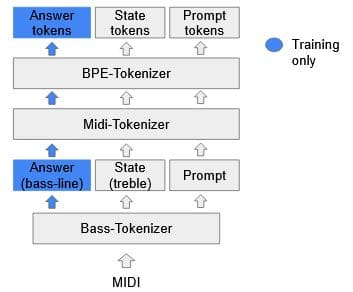
\includegraphics[width=0.5\textwidth]{IMAGES/Preprocessing1.jpg} 
    \caption{Preprocessing/tokenization of the original basscraft model}
    \label{fig:preprocessing1}
\end{figure}

\section{Comparing methods of adding control ca 1.5 months}
\subsection{Approach 1 - Vocabulary Extension}

Vocabulary expansion is the process to add new vocabulary to a transformer model. The method depends on several factors including which tokenizer is used, the set of new words and how it differs from the prior set. I.e is it a new language with no overlap, or a domain specific subset of a language where you may want to add common domain specific words.

In vocabulary expansion one maintains the prior tokenizer, to keep pretrained knowledge. 
The tokenizer used for the Basscraft model is a modified byte pair encoding (BPE) tokenizer \cite{Sennrich_Haddow_Birch_BPE_2016}, which is trained starting from a general alphabet, and greedily merges the most common pairs of tokens until the target vocabulary size is reached (16000). It is difficult to simply add new tokens here, as it would require retraining the BPE tokenizer, which will transform the embedding layer making it unusable. Common approaches are merging tokenizers, resizing the vocabulary to add new tokens while keeping the prior embeddings intact or replacing vocabulary items.
We choose vocabulary replacement of unused tokens with the new control tokens. This will inevitibally extend the sequence size, since the new tokens are not merged in the BPE process, which may adversly effect the model performance. However this will allow us to maintain the same embedding size, while still benefiting from the model's prior training. 

\begin{figure}[H]
    \centering
    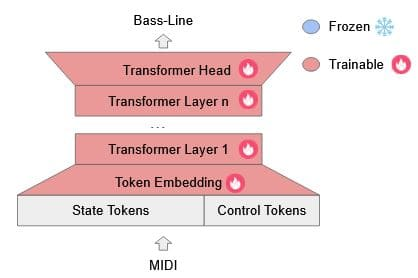
\includegraphics[width=0.5\textwidth]{IMAGES/full_ft.jpg}
    \caption{Vocabulary transfer with full  fine tuning}
    \label{fig:vocabtrans1}
\end{figure}

\begin{figure}[H]
    \centering
    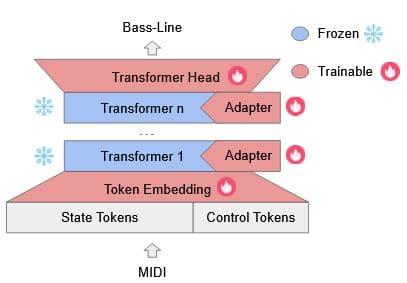
\includegraphics[width=0.5\textwidth]{IMAGES/vocab_lora_ft.jpg} 
    \caption{Vocabulary transfer with parameter efficient fine tuning}
    \label{fig:vocabtrans2}
\end{figure}

\subsection{Approach 2 - Integrating of control tokens} 

In this experiment we adjust the approach used in Coco-Mulla \cite{Lin_cocomulla_2024} inserting the embedded condition prefix into the last frozen layers of the model. The embedding is learnable. In contrast to the previous method we are not working with tokens as input tokens, we are incorporating them into the model after c layers. This method has the benifit that we don't need to worry about tokenisation and the vocabulary of the original model, as those remain unchanged. The difficulty is learning the embedding of the control tokens.
 
\begin{figure}[H]
    \centering
    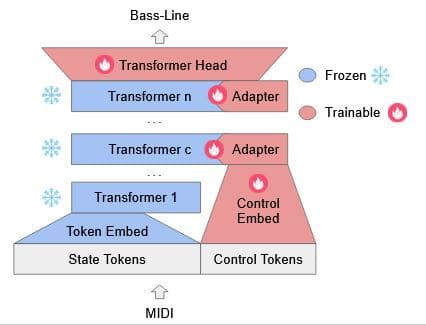
\includegraphics[width=0.5\textwidth]{IMAGES/ControlTokensLora.jpg} 
    \caption{Integration of control tokens with parameter efficient fine tuning}
    \label{fig:controltok}
\end{figure}

\subsection{Approach 3 - Post Hoc Conditioning}

This is the approach used by SMITIN\cite{Koo_Wichern_Germain_SMITIN_2024}. -> 

One potential problem: This may be very difficult to implement. SMITIN only has binary scenarios (presence of certain instruments), our current target variables are larger. What is nice about this approach is that it is very flexible, can be used in conjunction with other methods, and roughly emulates the guidance mechanisms used in diffusion models. 

\begin{figure}[H]
    \centering
    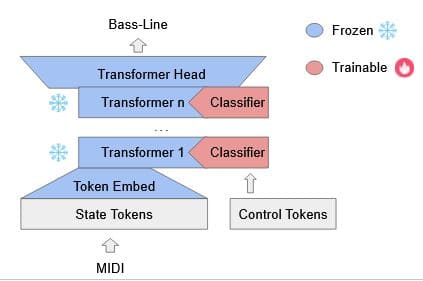
\includegraphics[width=0.5\textwidth]{IMAGES/adhoccontrol.jpg} 
    \caption{Integration of control using inference time interference}
    \label{fig:adhoccontrol}
\end{figure}

If these experiments are not successful, we can follow the approach of \cite{Shu_Xu_Musebarcontrol_2024} and try additional training using auxiliary tasks and using a modified (counterfactual) loss function. 

Other potential avenues to explore in this section (if time remains) is how controls stack. Adapters for the different target controls can be trained separately, then merged.  

\section{Application to larger model 1.5 months}

The first step in this experiment is extracting and tokenizing either spectral or inner metric weight which is then tokenized and passed to the MusicLang Llama 2 model. They will be integrated with the most successful method determined above.

\section{Integration into LastMinuteGig 2 months}
This project is motivated by extending the music engine of LastMinuteGig. \cite{Chalkiadakis_2022}. The application currently employs a very simple algorithm. I will outline it below. 
\begin{itemize}
    \item{1}: Randomly choose key, rhythmic pattern, chord progression and tempo from a pool of possible values.
    \item{2}: Play corresponding percussion audio clip (depends on tempo and rhythmic pattern)
    \item{3}: When user plays the button trigger the guitar sound of the current chord.
    \item{4}: After 8 bars - make a random change (to rhythm, tempo, pause)
\end{itemize}


This music engine will be changed in the following way. Most of the generative process will be done asynchronously.
\begin{itemize}
    \item{1}: Create $n=100$ musical pieces with different control settings
    \item{2}: For each piece
    \item{3}: Extract chords from prompt (assuming high control success) - save mapping $m1$
    \item{4}: Extract change of rhythmic pattern (or tempo or meter or instrumentation since these are already controllable in the musiclang model) - save mapping
    \item{5}: Render symbolic music to audio
\end{itemize}

During game play
\begin{itemize}
    \item{1}: Load random audio clip and mappings.
    \item{2}: Play associated guitar chords when player taps.
    \item{3}: Register changes in tapping on musical changes.
    \item{4}: Repeat when audio clip has finished playing.
\end{itemize}


This will be followed by a user study on healthy participants following the original protocol\cite{Chalkiadakis_2022}


\section{Thesis Timeline}

\begin{figure}[H]
    \centering
    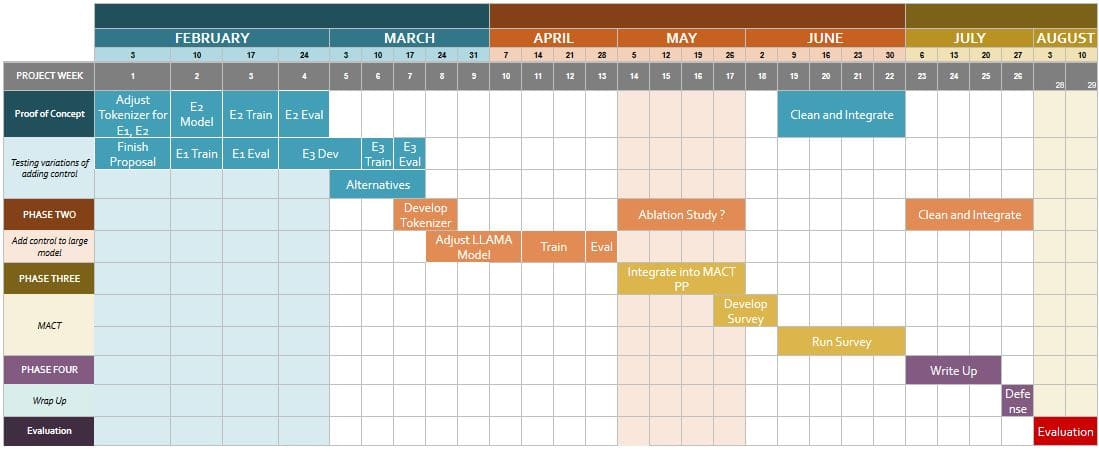
\includegraphics[width=1\textwidth]{IMAGES/project_plan.jpg} 
    \caption{Thesis project plan}
    \label{fig:projectplan}
\end{figure}


